% !TeX root = ../main/main.tex
\documentclass[../main/main.tex]{subfiles}

\begin{document}
\espacio

  El paradigma computacional ha cambiado bastante desde la comercialización de la computadora personal (PC) en 1981. El cofundador de Intel, Gordon E. Moore, planteó en el año 1965 el siguiente enunciado: ``El número de componentes de un circuito integrado duplicará cada dos años...'' \cite[p.~2]{article:ley_de_moore}.

  \begin{figure}[H]
    \centering
    \caption{Incremento del número de transistores por microprocesador}
    \fbox{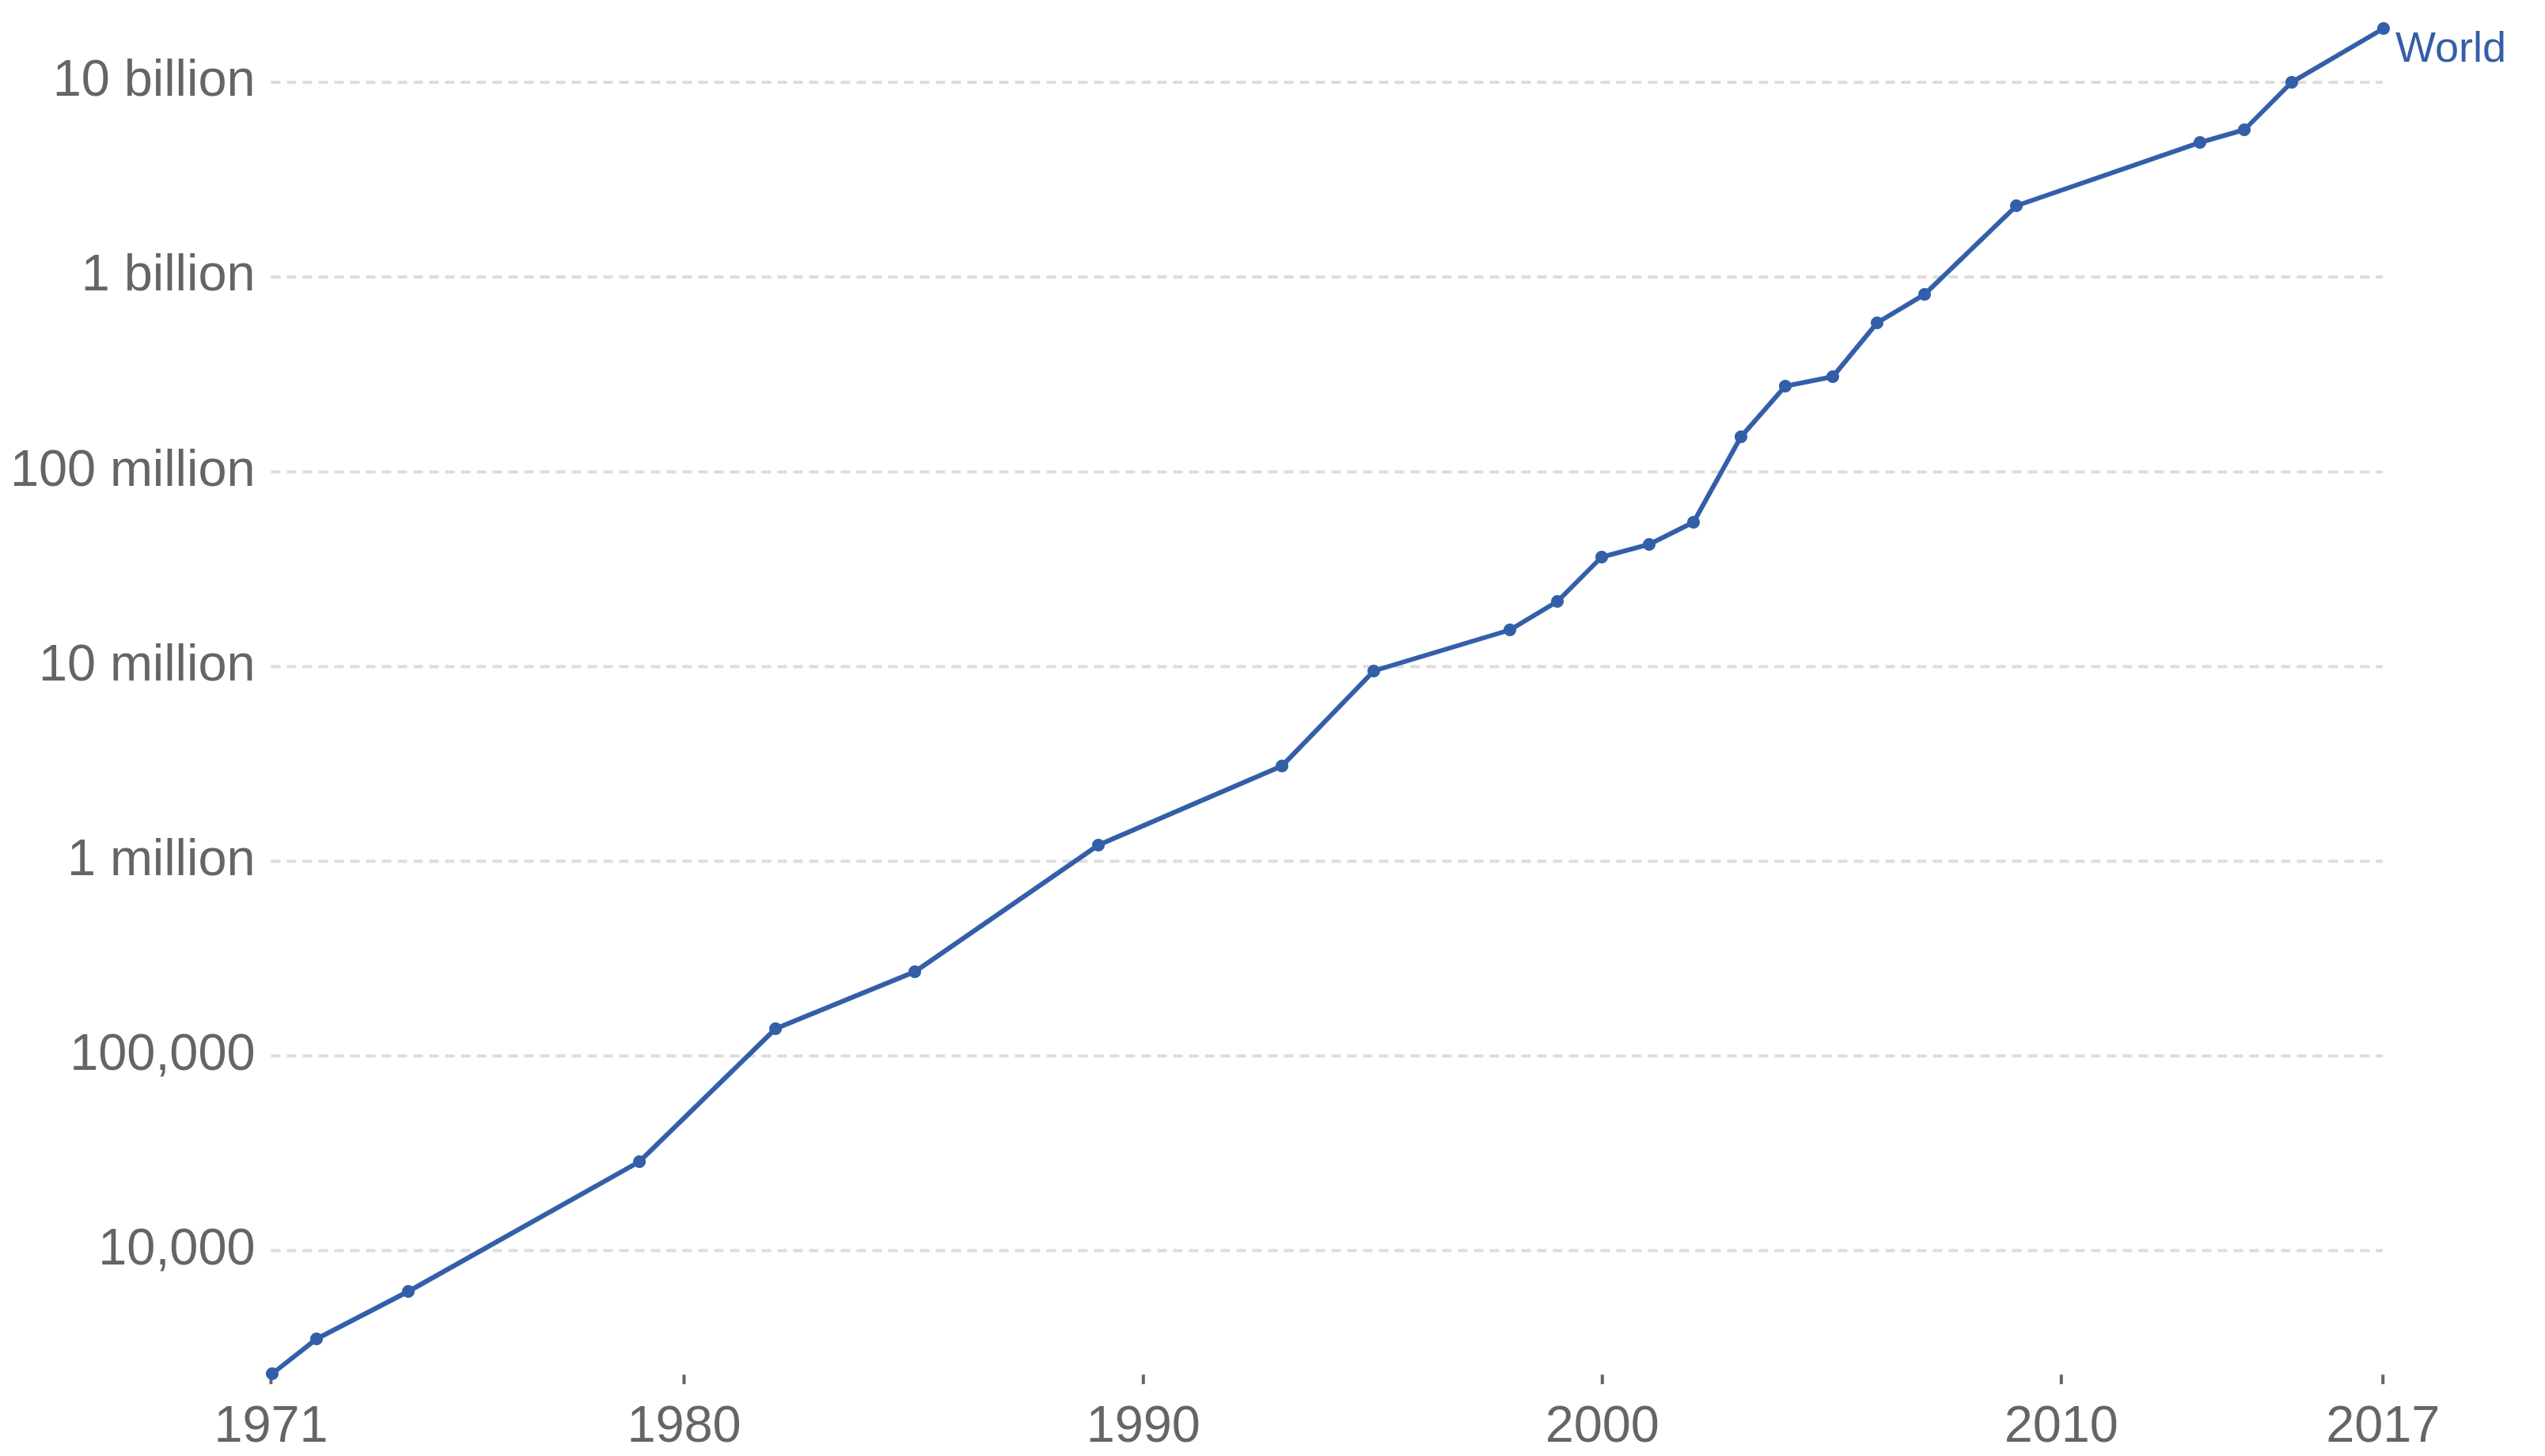
\includegraphics[width=13.5cm, keepaspectratio]{introduccion/transistores_por_microprocesador.png}}
    \caption*{\textbf{Fuente:} Rupp Karl. 40 Years of Microprocessor Trend Data. 2018. URL: \url{https://github.com/karlrupp/microprocessor-trend-data}. Consultado el 4 de Marzo de 2020.}
    \label{fig:transistors_microprocessor}
  \end{figure}

  Como se puede observar en la Figura \ref{fig:transistors_microprocessor}, esta ley empírica se cumplió hasta la actualidad. Sin embargo, tanto Stephen Hawking, como el propio Moore predijeron que esta ley dejaría de cumplirse entre los años 2017 y 2022 debido a los adelantos científicos de la microelectrónica, la velocidad de la luz y la naturaleza atómica de la materia.\footnote{The Inquirer Magazine, 19 de septiembre de 2007}

  La popularidad de los Dispositivos Inteligentes (Smart Devices), Accesorios Ingeligentes (Wearables) y el Internet de las Cosas (IoT), demuestra que los circuitos integrados han alcanzado un tamaño muy pequeño, el cual es complicado reducir aún más.

  El objetivo de la reducción de circuitos es el de incrementar la velocidad de procesamiento mediante el número de transistores por procesador, sin embargo, este proceso conlleva un cuantioso costo en la investigación de nuevas aleaciones, solución a los problemas de sobrecalentamiento y consumo de energía.

  Como una medida para evadir estos problemas, los fabricantes de microprocesadores cambiaron el paradigma del desarrollo de hardware de la arquitectura mono-núcleo a la arquitectura multi-núcleo. Después de este cambio se pudo observar que el límite del número de procesadores de uso general llegó a una cantidad difícil de superar debido al espacio físico que ocupan y al calentamiento de los circuitos, dado que la temperatura es inversamente proporcional al trabajo de cómputo que se designa a cada circuito; por ello muchas aplicaciones actuales hacen uso de recursos externos al procesador central para solucionar tareas específicas, un ejemplo común es el cómputo de matrices de pixeles de imágenes o videos, en arreglos que puden sobrepasar los 8.3 millones de elementos, este cómputo es realizado en tarjetas gráficas que procesan estos volúmenes gigantescos de datos y devuelven el resultado al procesador central o bien muestran el resultado en una o más pantallas.

  El Estándar de Encriptación Avanzada (AES Rijndael) es utilizado en muchas aplicaciones actuales debido a su característica de patrón abierto para uso público y privado en aplicaciones tanto personales, como empresariales.

  \begin{table}
    \centering
    \caption{Aplicaciones del algoritmo AES}
    \begin{tabular}{|p{6cm}|p{8cm}|}
  \hline
  \multicolumn{1}{|c|}{\textbf{USO}} & \multicolumn{1}{c|}{\textbf{APLICACIONES}}       \\ \hline
  Compresiòn de datos & 7z, Amanda Backup, PeaZip, PKZIP, RAR, WinZip, UltraISO 
  \\ \hline
  Encriptación de archivos & Gpg4win, Ncrypt
  \\ \hline
  Encriptación de particiones de disco duro & NTFS, BTRFS
  \\ \hline
  Encriptación de discos duros & BitLocker, CipherShed, DiskCryptor, FileVault, GBDE, Geli, LibreCrypt, LUKS, Private Disk, VeraCrypt
  \\ \hline
  Seguridad en comunicaciones LAN & CCMP, ITU-T G.hn, IPsec
  \\ \hline
  Seguridad en comunicaciones en Internet & GPG, TLS, SSL
  \\ \hline
  Otras aplicaciones & KeePass Password Safe, Pidgin, Google Allo, Facebook Messenger, WhatsApp
  \\ \hline
\end{tabular}
    \caption*{\textbf{Fuente:} Elaboración propia}
    \label{tabla_uso_aes}
  \end{table}

  El incremento en la velocidad de ejecución de algoritmos de cifrado llega a ser de gran utilidad, ya que, como se muestra en el cuadro \ref{tabla_uso_aes}, los protocolos SSL y TLS trabajan en base a la encriptación AES Rijndael; de acuerdo con las estadísticas de \emph{Google Referral URL}, un 85\% de servicios tanto de red local como de internet intercambian información cifrada; por tanto, la ejecución de este proceso debería ser veloz para reducir la latencia de las comunicaciones cifradas, incrementar la velocidad de la compresión de datos o del cifrado y descifrado de archivos.

  Observando el algoritmo de cifrado que utiliza el método del Estándar de Encriptación Avanzada (AES Rijndael), se puede concluir que este algoritmo es pasible a ser paralelizado en múltiples hilos de ejecución de procesos ya que en la mayor parte de este proceso se realizan cálculos aislados e independientes. Para realizar estos cálculos se plantea la delegación del algoritmo a la GPU (Unidad de Procesamiento Gráfico) a fin de reducir la carga de tareas asignadas a la CPU (Unidad Central de Procesamiento), evitando así las colas insostenibles de procesos e incrementando la velocidad de ejecución del algoritmo, llegando a establecer conclusiones y mostrando resultados que servirán como base para investigaciones posteriores referentes a la reducción de latencia en las comunicaciones cifradas.
\end{document}